\documentclass[11pt,oneside]{book}

\usepackage[paperheight=297mm,paperwidth=210mm,width=150mm,top=30mm,bottom=30mm,bindingoffset=10mm, inner=30mm, outer=25mm]{geometry}
\usepackage[utf8]{inputenc}
\usepackage{graphicx}
\usepackage{caption}
\usepackage{subcaption}
\usepackage[nottoc]{tocbibind}
\usepackage{datetime}
\usepackage[colorlinks]{hyperref}
\usepackage{fancyhdr}
\usepackage{setspace}
\usepackage{kotex}
\usepackage{amsmath}
\usepackage{booktabs}
\usepackage{multirow}
\usepackage{tabularx}
\usepackage{rotating}
\usepackage{titlesec}
\usepackage{tocloft}
\usepackage[acronym,nomain,nonumberlist]{glossaries}
\usepackage[table]{xcolor}
\usepackage[toc,page]{appendix}
\usepackage{pdfpages}
\usepackage{svg}
\usepackage{longtable}
\usepackage[english]{babel}
\usepackage{blindtext}
\usepackage{float}

%Add acronyms if necessary
\makeglossaries
\newacronym{usj}{USJ}{University of Sri Jayewardenepura}
\newacronym{foe}{FOE}{Faculty of Engineering}

\setcounter{secnumdepth}{4}

%Copy all the images to images folder
\graphicspath{ {images/} }

%for print
%\hypersetup{citecolor=black, filecolor=black, linkcolor=black, urlcolor=black}
%for electronic
\hypersetup{citecolor=black, filecolor=black, linkcolor=black, urlcolor=blue}

\newdateformat{monthyeardate}{\monthname[\THEMONTH] \THEYEAR}
\pagestyle{fancy}
\fancyhead{}
\fancyhead[RO,LE]{\nouppercase{\leftmark}}
\renewcommand{\headrulewidth}{0.4pt}

\renewcommand{\cftfigpresnum}{Figure\ }
\newlength{\mylenf}
\settowidth{\mylenf}{\cftfigpresnum}
\setlength{\cftfignumwidth}{\dimexpr\mylenf+2.5em}
\setlength{\cfttabnumwidth}{\dimexpr\mylenf+1.8em}
\newcolumntype{C}[1]{>{\centering\let\newline\\\arraybackslash\hspace{0pt}}m{#1}}
\usepackage{hyperref}
%%%%%%%%%%%%%%%%%%%%%%%%%%
%% Document begins here %%
%%%%%%%%%%%%%%%%%%%%%%%%%%
\begin{document}

\pagenumbering{gobble}
\begin{titlepage}
    \begin{center}
        \vspace*{0cm}
        
        \begin{figure}[h]
        \begin{center}
        
\includegraphics[width=.3\columnwidth]{image/Logofrauas.png}
        \end{center}
        \end{figure}
        \vspace*{1cm}
        
        \vspace{1cm}       
        {\Large \textbf{Frankfurt University of Applied Sciences}}
        \vspace{1cm}
        
        {\Large \textbf{High Integrity System}}
        \vspace{1cm}
        
        \LARGE
        \textsc{Advanced Real-Time Systems}
        \vspace{1cm}
                
        \Huge
        \textbf{Real-time Postbox Notification}
        \vspace{1.5cm}
        
        
        \large 
        Supervise by
        \vspace{.3cm}
        
        \Large 
        Prof. Dr. Ing. Matthias Deegner
        \vspace{1cm}
        
        \setstretch{1.5}
        
        \large 
        Submitted by
        \vspace{.3cm}
        
        \LARGE
        Parth Desai (1381870)
        \\Hardikkumar Dudhat (1381870)
        \\Milankumar Goti (1381867)
        \vspace{0.5cm}

        
     
        \vfill
        {\small \monthyeardate\today}
        
            
        \vspace*{0cm}
        
    \end{center}
\end{titlepage}
 %\pagenumbering{gobble} if we need to remove page numbering

%\setstretch{1.0}
%\chapter*{Acknowledgements}
%\pagenumbering{roman} %Start Roman page numbering
%\setstretch{1.5}
%\input{acknowledgements}
%\setstretch{1.0}

\clearpage
\newpage
\tableofcontents
\newpage
\listoffigures
\glsaddall

\setstretch{1.0}
\chapter*{Abstract}
\pagenumbering{arabic}%Start Arabic page numbering
\setstretch{1.5}
\label{Abstract}
Since most multi-story buildings such as apartments, condominiums, office buildings, etc have a centralized post-box location, users are limited on how often they can visit to check or collect their post. In order to determine whether they have any new posts or letters in their post-box, they must periodically check it speculatively. Most users neglect to check their post boxes. As a consequence, sometimes important letters go unnoticed, resulting in various miseries. Since official letters are becoming more widely used worldwide due to their high level of confidentiality, users are seeking a better solution that will keep them on their toes when receiving posts. The goal of this project is to create a smart post-box. In this case, the post-box is designed to notify the recipient when a post has been delivered and to provide access to the right person. This project used an ultrasonic sensor, which is connected to NodeMCU, that is used to detect objects inside the post-box, SMTP which is used to notify users about the new arrival of a post in the post-box by email, and Firebase which is used to store real-time data of distance between sensor and object. 

\setstretch{1.0}
\chapter{Introduction}
\setstretch{1.5}
\label{chapter:introduction}

The trend of home automation is on the rise in today's world. From energy-saving applications to fancy lighting controls, home automation has become a global phenomenon. It's human nature to look for the easiest solution. This attitude promotes innovation and productivity \cite{hassan_2018}. Mail is part of the postal system that delivers written documents in the form of envelopes and small parcels to recipients all over the world. In the late 1990s, e-mail dominated the mailing system since it was faster and cheaper than the postal service and enabled users to communicate worldwide. Nonetheless, most of our vital documents and official documents are sent in the conventional manner which is our postal system \cite{Subramaniam2007}.

The existence of electronic mail (e-mail) has caused most people to forget to check their physical post-box. Additionally, because of their busy lives, people do not have time to check their post-box regularly. Oftentimes, these situations have led to the loss of important notices or mails and even cause them to become insensitive to the presence of such notices in the first place \cite{Muhamaad_2019}.

Smart Post-box has found a new revolution in using newer technologies to alert the users on the event a mail is delivered, especially through e-mail.

\section{Objectives}
This project was implemented based on a review of current mail boxing approaches.
Users frequently lose and leave mail sent and placed in mailboxes. The major objective of this project is to notify the owner of the post-box. Specific objectives are: 

\begin{itemize}
  \item To collect the data from the ultrasonic sensor and send it to the micro-controller unit, which is NodeMCU.
  \item To update the data in the Firebase.
  \item To trigger an event based on distance.
  \item Finally, the owner should be notified by sending an email if the measured distance is less than 8.
\end{itemize}

\setstretch{1.0}
\chapter{State of Art}
\setstretch{1.5}
\label{chapter: State of Art}

In this section, we've looked at some of the previous trials and detailed some of the methodologies and operational ideas that were employed.

Supraja C D and Bindusree V created namely making bell notifications which are used to help deaf people to respond to bell sounds. In this study, the message will be sent via a wireless module, with one module installed on the doorbell, and the other module will be connected to the user, with several LED/vibration motors installed as an indication so that the LCD screen will display text for notification purposes. The Arduino Control Unit controls these modules \cite{devi2019}.

Lidzatus S created a doorbell whose purpose is to help solve some of the problems that occur in everyday life, especially for hosts who don't hear the sound of the bell because they have problems hearing or don't hear the sound of the bell because they are playing a gadget complete with earphones, this system is designed by using the wifi module Node-MCU ESP8266 as a control to send notifications to e-mail \cite{setiawan2021}.

Bindu Sebastian, Mashitha, and Meghana created a project named an intelligent mailbox system that is capable of automatically sending information about mail to users and delivering notifications to courier officials using GSM and RFID technology. They have used a dc motor for opening and closing a mailbox, so it can provide security to the system \cite{Sebastian2016}.

The Smart system letterbox was developed by Anjali Devi Pujari, Priyanka Bansode, Pragati Girme, Harshal Mohite, and Anirudha Pande, in which a hardware kit alerts the user that a letter has arrived. Notifications are received through the mobile application. The obstacle sensor is used to identify objects (letters). Using the RTC clock, the delivery time of the letter can be stored. Through the GSM module, the notification is sent by message and the GPS module detects the location at which the letter has been received \cite{Bansode2016}.

Siva Kumar Subramaniam, Siti Huzaimah Binti Husin, Yusmarnita Binti Yusop, Abdul Hamid bin Hamidon created a Real-time mailbox alert system via SMS or email in that this system, Mails delivered into the user’s mailbox, the system will automatically generate an alert which is sent in the form of a short message system or email that typically details the real-time of mail delivery. The system is designed to ease human life by sending SMS or email to notify the user about important new mails reaching the user’s mailbox \cite{Subramaniam2007}.


\setstretch{1.0}
\chapter{Method and Material}
\setstretch{1.5}
\label{chapter:Methods and Materials}
In this project, we have used NodeMCU, an Ultrasonic sensor, Firebase real-time database, and an SMTP mail function.

\section{Analysis}
One of the main function of our project is e-mail notification. As there are several mail transfer protocols such as SMTP(Simple Mail Transfer Protocol), POP(Post Office Protocol), and IMAP(Internet Message Access Protocol), we have find best method for mail transfer. 

\subsection{Comparison of SMTP, POP, and IMAP}
The Simple Mail Transfer Protocol (SMTP) is a protocol that mail servers use to send, receive, and/or relay email between senders and receivers. The address (or addresses) of an SMTP email server can be set by the mail client or application you're using, and is usually formatted as smtp.serveraddress.com.

The most significant distinction between these protocols is that SMTP is the only protocol that allows you to transmit, or "push," email from one unknown mail server to another. POP and IMAP are email protocols for receiving or "pulling" messages from a recipient's own mail server. As a result, POP and IMAP only allow mail to be sent to confirmed mail servers. They can't be used outside of your own networks for communication \cite{Goud2020}.

POP is a message access protocol, whereas SMTP is a message transfer protocol. To put it another way, SMTP is used to transmit mail from one user to another, and POP is used to receive mail. SMTP is used twice: once to establish the connection and send data between the sender and the email server, and again to send data and connect to the receiver. Between the receiver and their mail server, POP is only utilized once \cite{Tzerefos1997}.

IMAP is a message access protocol, whereas SMTP is a message transfer protocol. IMAP simply fetches messages and handles incoming email, whereas SMTP transmits messages and handles outgoing email \cite{kara2019}.

With SMTP, we will receive helpful delivery information regardless of what happens to your email after you send it. You can check to verify if your messages were sent to the intended recipient and look for any problem codes \cite{Bettina2022}.

Another benefit of running your own SMTP is that email list is not being shared with anyone, ensuring the data privacy of company and customer \cite{Bettina2022}.

\section{Modelling}
\subsection{Modelling Post Detection}
Modeling is used to obtain the desired functionality of the Post detecting system. The smart postal mailbox is a system for determining the presence of posts in a mailbox from a remote location regardless of distance, consisting of a sensor for detecting the presence of post in a mailbox, while the sensor is positioned in the mailbox; a control unit that communicates with the mailbox sensor and is used for storing information of the mailbox status, while the status is used for observation. Following are the most signification functions:
\begin{itemize}
    \item detecting the presence of a consignment in the mailbox
    \item collecting time data about deliveries,
    \item storing data in the database,
    \item ensuring communication between database and NodeMCU
\end{itemize}

\subsection{Modelling User Notification}
The real-time mail alert system is a device that helps users by providing real-time notifications when new mail arrives, replacing the usual method of monitoring mail. User will get notified, with aid of header file 'ESP\textunderscore Mail\textunderscore Client.h' and implementing SMTP mail function.

\section{Tools and Technologies}
In the creation of this real-time post box notification, we employed the following hardware, and Technologies which is listed below.

\subsection{NodeMCU ESP8266}
A microcontroller unit, which is a small computer, is housed on a single metal-oxide-semiconductor integrated circuit chip. A microcontroller is a device with one or more CPUs, memory, and programmable input/output peripherals that can be used to connect miniature screens, buttons, motors, and sensors, among other things. A microcontroller may be programmed and controlled. The microcontroller's primary duty is to connect to WiFi and then to the Firebase. The microcontroller has been configured to connect to both WiFi and the Firebase. As a result, the data from the ultrasonic sensor is used to compare the distances, and an event is triggered in the Firebase as a result \cite{Shakthidhar2019}.
\begin{figure}[htp]
    \centering
    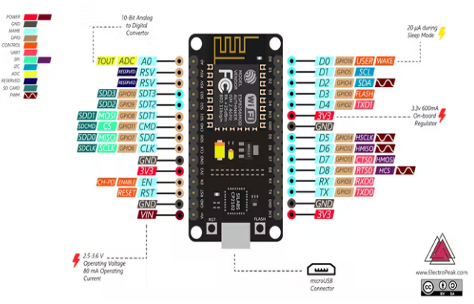
\includegraphics[width=12cm]{image/NodeMCU.png}
    \caption{NodeMCU \cite{NodeMCUIMG}.}
    \label{fig:NodeMCU}
\end{figure}

\subsection{HC-SR04 Sensor (Ultrasonic Sensor)}
The HC-SR04 is a low-cost, simple-to-use distance measuring sensor with a range of 2 to 400 cm (about an inch to 13 feet). Two ultrasonic transducers make up the sensor. One is the transmitter, which generates ultrasonic sound pulses, and the other is the receiver, which detects reflected waves. You may compute the distance by taking into account the travel time and the sound's speed. The Trig pin must be set to High State for 10 seconds in order to create the ultrasonography. This will cause an 8-cycle ultrasonic burst to be sent out, which will travel at the speed of sound. After those 8 cycles, an ultrasonic burst is sent, the Echo pins go high right immediately, and it begins listening or waiting for that wave to be reflected from an item. If no object or reflected pulse is present, the Echo pin will time out after 38 milliseconds and return to its low state. The Echo pin will travel down faster than those 38ms if we receive a reflected pulse. We can determine the distance traveled by the sound wave based on the length of time the Echo pin was HIGH, and thus the distance from the sensor to the item \cite{Dimitrov2016}.
\begin{figure}[htp]
    \centering
    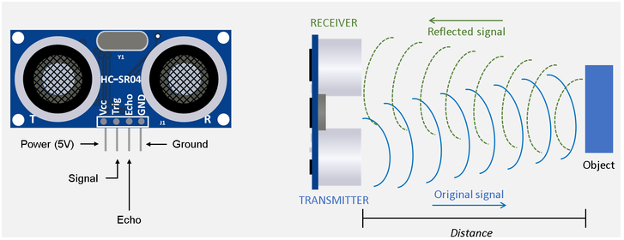
\includegraphics[width=12cm]{image/ultrasonic_sensor.png}
    \caption{Ultrasonic sensor \cite{ultrasonicIMG}.}
    \label{fig:ultrasonic}
\end{figure}

\subsection{Firebase Database}
Firebase, which is owned by Google, is a real-time database stored on the cloud. It distributes a real-time database instance to each connected client and ensures that they receive real-time updates with the most recent data. It saves data in JSON format and allows for cross-platform scripting. In terms of the scope of our prototype, it saves all users' unique IDs, login credentials, device state information, and usage duration \cite{Moroney2017}.

\section{Implementation}
In our project we have implemented hardware as well as software side in form of cloud database and email function.
\subsection{Hardware Implementation}
The hardware implementation of the system is very straightforward, as it has only two components, one is NodeMCU, and another is an ultrasonic sensor.

First of all, an ultrasonic sensor is connected to NodeMCU. Trigger pin and Echo pin are connected to two GPIO of NodeMCU and ground and Vcc are connected with its related pin.

After that, NodeMCU is connected with a remote power supply such as a 9V battery or power bank. 
\begin{figure}[htp]
    \centering
    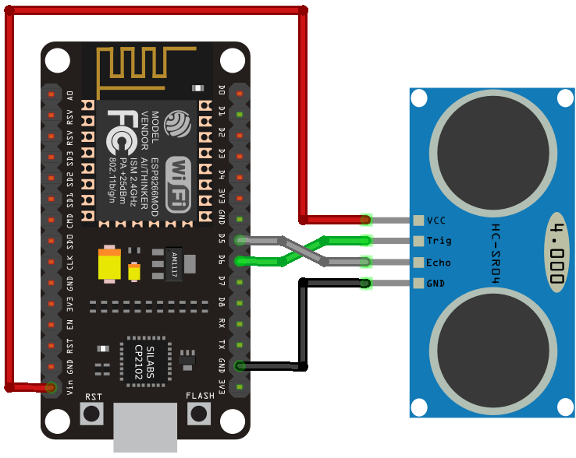
\includegraphics[width=10cm, height=8cm]{image/Circuit_diagram.png}
    \caption{Circuit diagram}
    \label{fig:circuit_diagram}
\end{figure}

\subsection{Software Implementation}
The Software side of our project includes mainly Firebase database and SMTP mail function.

\textbf{Firebase Implementation}, we have created a new database with relevant fields along with a distance field, which is most important because this field will be updated every time the post-box receives a new post.

\textbf{Distance Function}, it measures the distance between the sensor and the post-box door. A limit is set to 8. The Trig (Trigger) pin triggers the ultrasonic sound pulses. The echo pin generates a pulse when it receives the reflected signal. Based on the measured duration distance variable is calculated. 

\textbf{Storing real-time data}, for this we must include header file 'FirebaseESP8266.h' to connect NodeMCU to the Firebase. The variables used and seen in Fig.~\ref{fig:firebaseauth} are: 
\begin{itemize}
    \item API\textunderscore KEY - identify your Firebase project
    \item DATABASE\textunderscore URL – URL of the database
    \item USER\textunderscore EMAIL – Email of user’s Firebase account
    \item USER\textunderscore PASSWORD – Password of user’s Firebase account
\end{itemize}

\begin{figure}[htp]
    \centering
    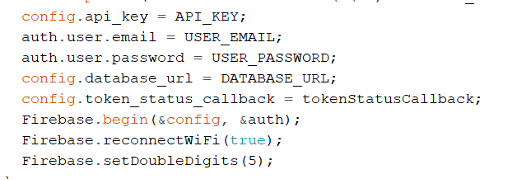
\includegraphics[width=12cm]{image/firebase-auth.png}
    \caption{Snippet - Firebase auth}
    \label{fig:firebaseauth}
\end{figure}

\textbf{Notifying users}, the user will get notified by email when a new post arrives in the post-box. For this, we set a predefined condition, if the distance is less than 8 then using the SMTP mail function user will get notified by email. A header file that should be included for the mail function is ESP\textunderscore Mail\textunderscore Client.h. The variables used are: 
\begin{itemize}
    \item SMTP\textunderscore HOST- Server name
	\item SMTP\textunderscore PORT - A communication endpoint that handles the transfer of email data over SMTP 
	\item AUTHOR\textunderscore EMAIL – Sender’s email address
	\item AUTHOR\textunderscore PASSWORD – Sender’s password for the particular email address
	\item RECIPIENT\textunderscore EMAIL – Receiver’s email address.
\end{itemize}

Fig.~\ref{fig:SMTPmail} shows a code snippet for notifying the users by email regarding the new arrival of post.
\begin{figure}[htp]
    \centering
    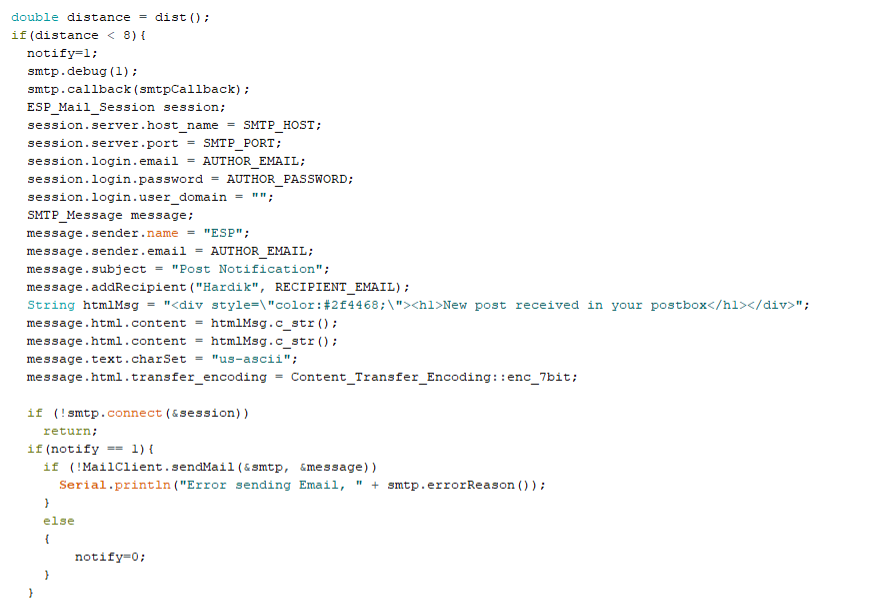
\includegraphics[width=14cm, height=13cm]{image/SMTP_mail.png}
    \caption{Snippet - SMTP mail}
    \label{fig:SMTPmail}
\end{figure}

\section{Flow Diagram}

First of all, we initialize the ultrasonic sensor by providing power. Now ultrasonic sensor transmits rays and distance will be calculated frequently. If the distance is less than 8 that means a new post arrived in the post-box and NodeMCU sends this distance data to Firebase and stores it there. After this SMTP mail function gets called and the user gets a notification about the arrival of a new post. Otherwise, it measures distance continuously. 
\begin{figure}[htp]
    \centering
    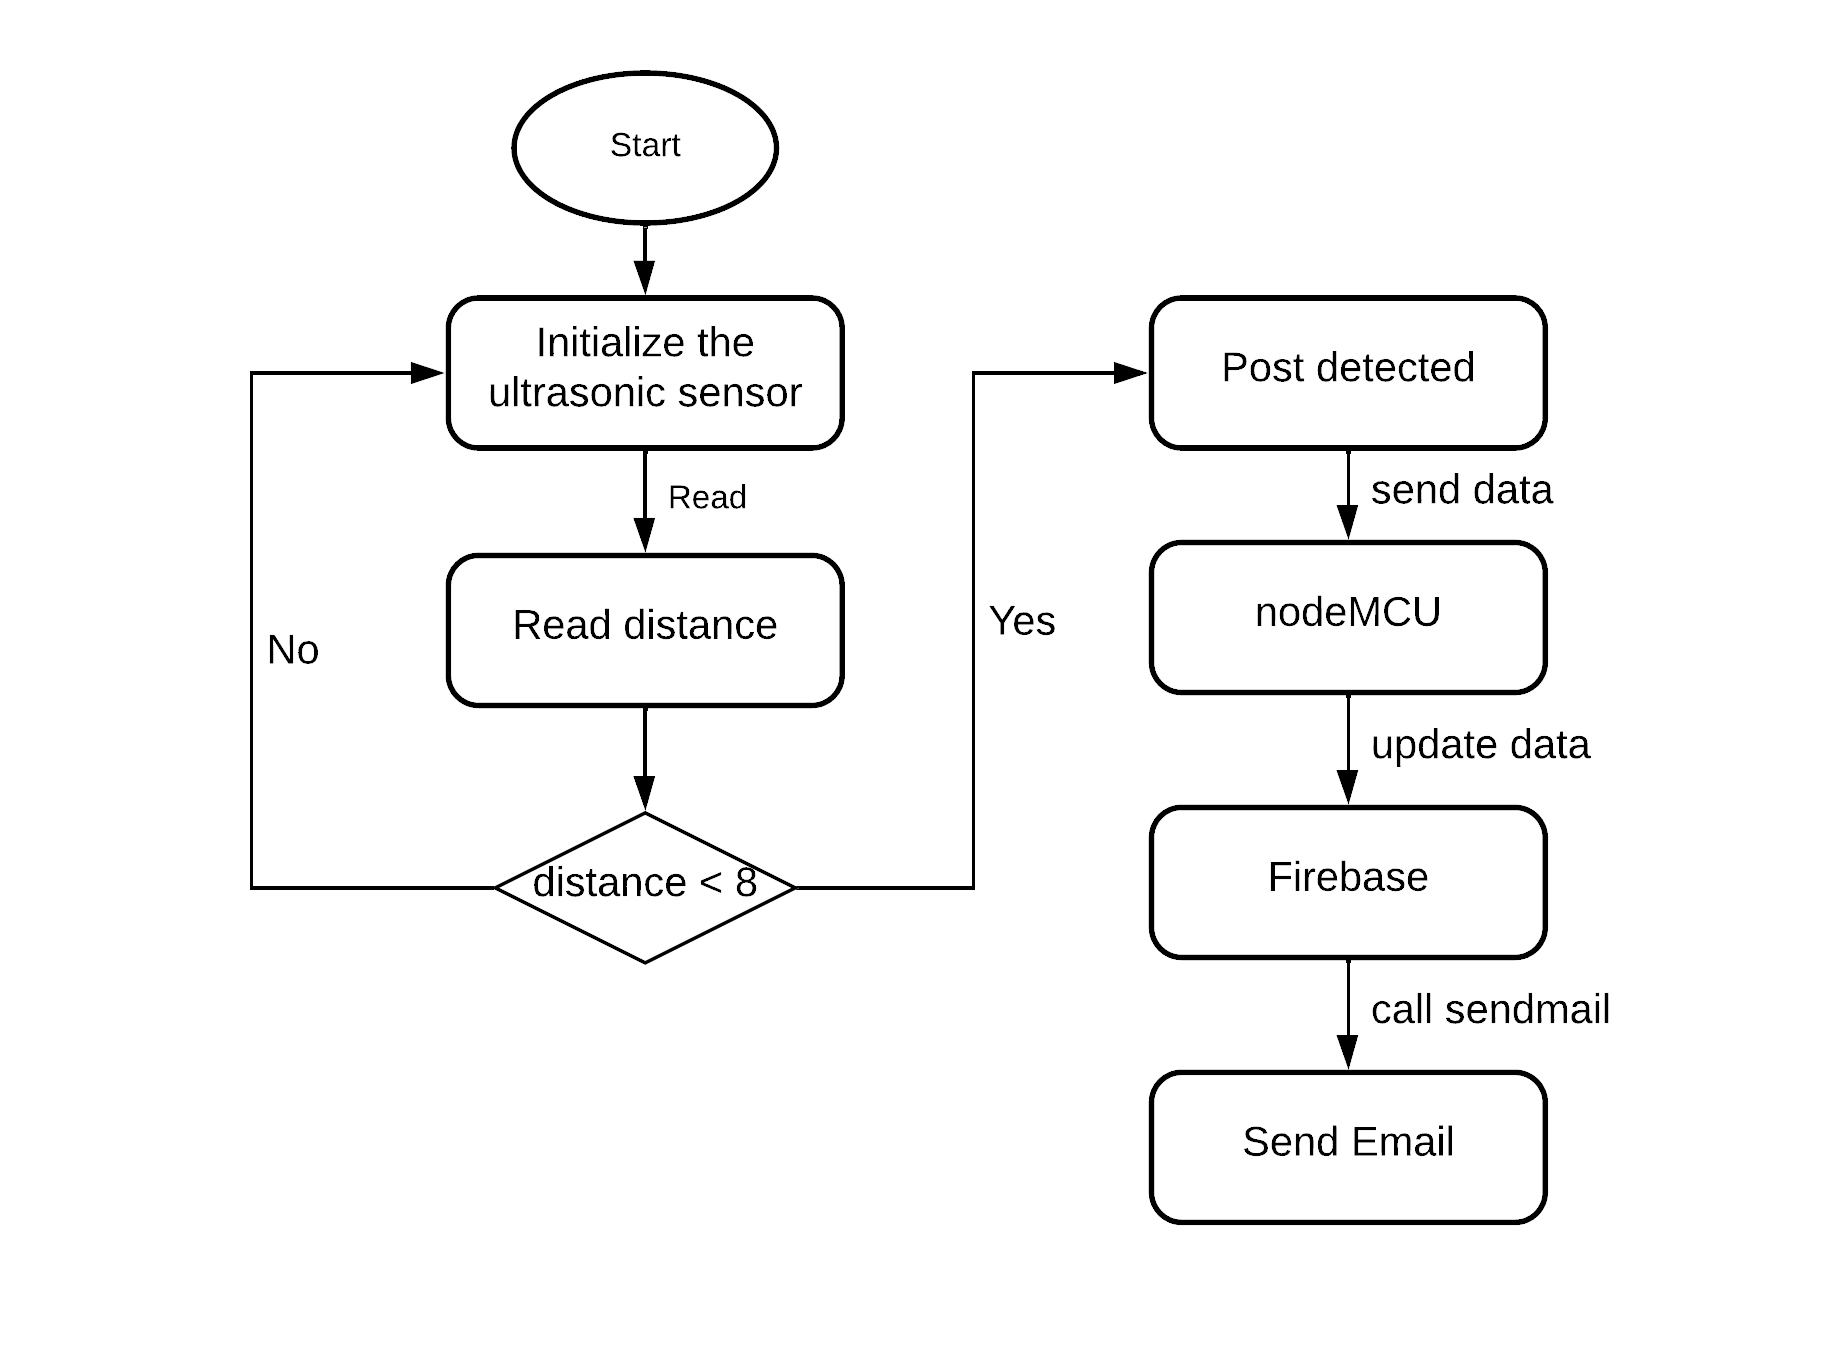
\includegraphics[width=12cm]{image/HCI.png}
    \caption{Snippet - SMTP mail}
    \label{fig:Flowchart}
\end{figure}\\
We have uploaded the source code along with a video of the running prototype, and source code of Latex on GitHub. \textbf{\href{https://github.com/hardik1111/Real-Time-Postbox-Notification}{https://github.com/hardik1111/Real-Time-Postbox-Notification}}:


\setstretch{1.0}
\chapter{Results}
\setstretch{1.5}
\label{chapter: Results}
This project has been focused on creating a system of smart post-box and we have introduced the low-cost prototype of smart post-box which is designed to send an email notification for delivering posts and letters. 
\begin{figure}[htp]
    \centering
    \subfloat[connection]{{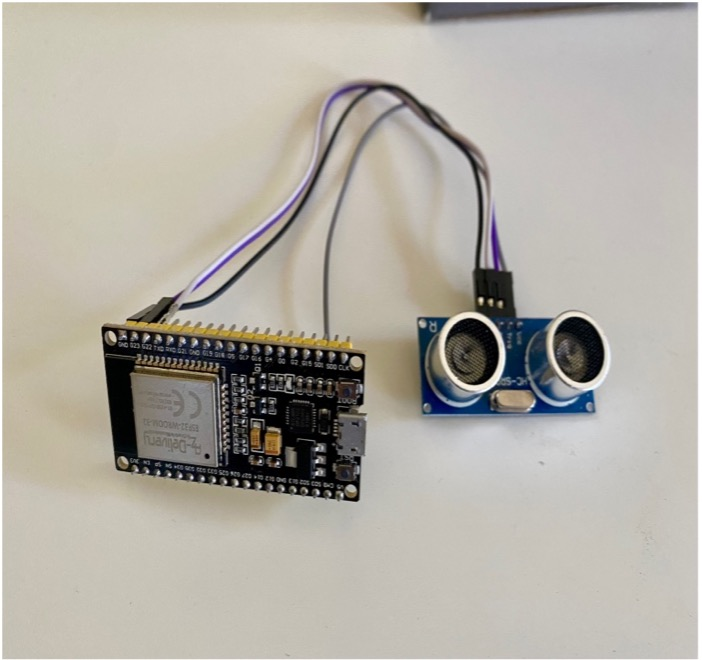
\includegraphics[width=6.5cm]{image/connection.jpg} }}
    \qquad
    \subfloat[postbox]{{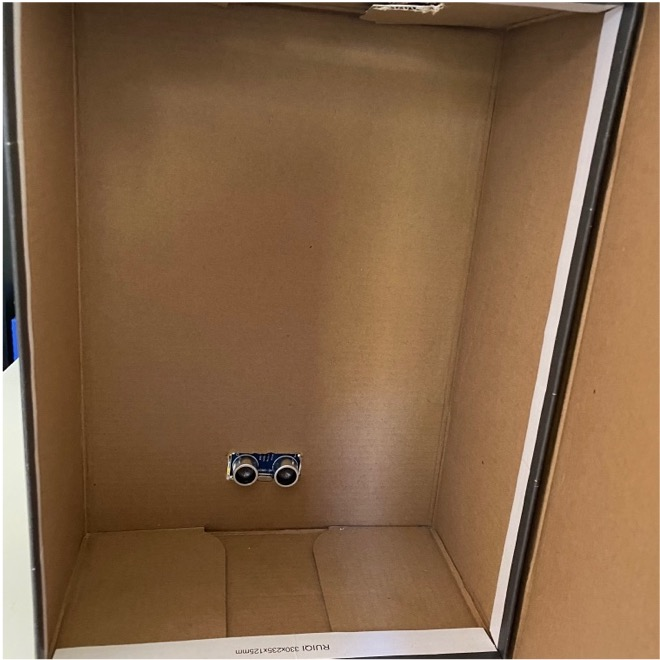
\includegraphics[width=6.5cm]{image/postbox.jpg} }}
    \caption{Final prototype}
    \label{fig:prototype}
\end{figure}

The objectives of the project have been met adequately with a bit of trial method. As soon as the Post-box receives the post, distance measure by the ultrasonic sensor will be greatly reduced, and through the NodeMCU firebase receives the data and an e-mail notification will be sent within a few seconds.  


\setstretch{1.0}
\chapter{Future scope}
\setstretch{1.5}
\label{chapter:Future Scope}
Although the prototype of the smart postbox works as per expectation, the ability of its usefulness can be enhanced further with some additional module implementation and careful coding logic.

First of all, at this point, we have only one way of notifying the user which is e-mail, but we can also implement an SMS service, which can be added via the GSM module or third-party services can be also used.

In the upcoming days, our proposed system will be implemented with a GUI interface inform of application and website, which will show all the related data such as time of incoming post and counter of posts. 

Furthermore, our algorithm is very naive, sometimes it cannot comprehend the availability of two posts at the same time, it gives faulty readings. Along with there are many real-life scenarios that we have overlooked such as, if a user only takes out only one of many posts, this will also create distance change and the system will give new post notification without having one. 

Lastly, one issue is that we have used a NodeMCU module for connection which requires the internet for working properly. This problem could be mitigated by using the GSM module. While this set of technology has its own problem It fulfills the current objectives. 

\setstretch{1.0}
\chapter{Conclusions}
\setstretch{1.5}
\label{chapter:Conclusion}

As smartphones and computers are very common gadgets for one’s daily life. IoT is not just a concept anymore, it is already a major part of our lives, and it is getting more and more involved in our lives, and with this project, it will help us in the future.

The Smart post-box with real-time email notification is designed such that users will be notified as soon as a new post arrives. The entire real-time system works as data is received from the ultrasonic sensor located inside of the mailbox. As the new post is detected by the ultrasonic sensor, the NodeMCU transmits the data to the Firebase database and an email notification is sent via the SMTP mail function. We have used SMTP because it has no sending volume limit and fully monitors email delivery, although it consumes more time, money, and effort for a small-scale project, we can ignore this disadvantage. As e-mail has become an integral part of everyone’s day-to-day life this system will provide users with various benefits.


\setstretch{1.0}
\bibliographystyle{ieeetrans}
\bibliography{references} %copy all references to references.bib file

%remove if 
\end{document}
